%=====================================================================
%  ISO8007 MSc Business Analytics Dissertation — Working Draft v1.0
%  Kartikey Sharma | 250559280 | Newcastle University Business School
%  Styling: Elsevier single-column journal format (cf. Yao et al., 2025,
%  Transportation Research Part F), adapted to ISO8007 submission rules
%  (1.5 line spacing, numbered pages, chapter-numbered tables/figures).
%=====================================================================
\documentclass[11pt,a4paper]{article}
\usepackage[T1]{fontenc}
\usepackage[utf8]{inputenc}
\usepackage{mathptmx}
\usepackage[scaled=0.90]{helvet}
\usepackage[left=2.4cm,right=2.4cm,top=2.3cm,bottom=2.4cm]{geometry}
\usepackage{microtype}
\usepackage{booktabs}
\usepackage{longtable}
\usepackage{array}
\usepackage{tabularx}
\usepackage{ragged2e}
\usepackage{graphicx}
\usepackage{xcolor}
\usepackage{tikz}
\usetikzlibrary{arrows.meta,positioning,calc,fit,backgrounds}
\usepackage{caption}
\usepackage{enumitem}
\usepackage{setspace}
\usepackage{fancyhdr}
\setlength{\headheight}{14pt}
\usepackage{float}
\usepackage{titlesec}
\usepackage[hidelinks]{hyperref}
\usepackage{amssymb}
\usepackage{amsmath}
\numberwithin{figure}{section}
\numberwithin{table}{section}

%---------------------------------------------------------------- colours
\definecolor{citeblue}{RGB}{0,102,153}
\definecolor{nublue}{RGB}{0,45,114}
\definecolor{nugrey}{RGB}{90,90,90}
\definecolor{rulegrey}{RGB}{150,150,150}
\definecolor{boxfill}{RGB}{243,246,250}
\definecolor{accent}{RGB}{158,27,50}

%---------------------------------------------------------------- captions
\captionsetup[figure]{font=small,labelfont=bf,labelsep=period,justification=justified,
  singlelinecheck=false,name=Fig.}
\captionsetup[table]{font=small,labelfont=bf,labelsep=newline,justification=justified,
  singlelinecheck=false,skip=3pt}

%---------------------------------------------------------------- headings
\titleformat{\section}{\normalfont\large\bfseries}{\thesection.}{0.6em}{}
\titleformat{\subsection}{\normalfont\normalsize\bfseries\itshape}{\thesubsection.}{0.6em}{}
\titleformat{\subsubsection}{\normalfont\small\bfseries}{\thesubsubsection.}{0.6em}{}
\titlespacing*{\section}{0pt}{14pt}{6pt}
\titlespacing*{\subsection}{0pt}{11pt}{4pt}
\titlespacing*{\subsubsection}{0pt}{9pt}{3pt}

%---------------------------------------------------------------- layout
\setlength{\parindent}{1.2em}
\setlength{\parskip}{0pt}
\onehalfspacing
\renewcommand{\arraystretch}{1.12}

\pagestyle{fancy}
\fancyhf{}
\fancyhead[L]{\footnotesize\itshape K. Sharma}
\fancyhead[R]{\footnotesize\itshape ISO8007 Dissertation, Newcastle University Business School (2026)}
\fancyfoot[C]{\small\thepage}
\renewcommand{\headrulewidth}{0.4pt}
\renewcommand{\headrule}{\hbox to\headwidth{\color{rulegrey}\leaders\hrule height \headrulewidth\hfill}}

%---------------------------------------------------------------- helpers
\newcommand{\ct}[1]{\textcolor{citeblue}{#1}}          % hyperlink-style citation
\newcommand{\xref}[1]{\textcolor{citeblue}{#1}}         % internal cross-reference
\newcolumntype{L}[1]{>{\RaggedRight\arraybackslash}p{#1}}
\newcommand{\placeholder}[2]{%
\begin{center}
\begin{tikzpicture}
\node[draw=accent,dashed,line width=0.9pt,fill=boxfill,rounded corners=2pt,inner sep=8pt,
 text width=0.93\textwidth]{\small\textbf{\color{accent}[TO BE COMPLETED --- #1]}\\[3pt]\small #2};
\end{tikzpicture}
\end{center}}
\newcommand{\notebox}[2]{%
\begin{center}
\begin{tikzpicture}
\node[draw=nublue,line width=0.8pt,fill=boxfill,rounded corners=2pt,inner sep=8pt,
 text width=0.93\textwidth]{\small\textbf{\color{nublue}#1}\\[3pt]\small #2};
\end{tikzpicture}
\end{center}}

\begin{document}

%=====================================================================
%  JOURNAL-STYLE FRONT MATTER
%=====================================================================
\thispagestyle{empty}
\begin{center}
{\color{rulegrey}\rule{\textwidth}{0.8pt}}\\[3pt]
\begin{minipage}{0.30\textwidth}\centering
{\footnotesize\sffamily\color{nublue}\textbf{NEWCASTLE}\\\textbf{UNIVERSITY}\\\textbf{BUSINESS SCHOOL}}
\end{minipage}%
\begin{minipage}{0.44\textwidth}\centering
{\footnotesize Dissertation submitted in part fulfilment of}\\[2pt]
{\large\itshape MSc Business Analytics}\\[3pt]
{\footnotesize Module ISO8007 \textbullet{} Academic Year 2025/26}
\end{minipage}%
\begin{minipage}{0.24\textwidth}\centering
{\footnotesize\color{nugrey} Working Draft v1.0\\ 18 August 2026}
\end{minipage}\\[3pt]
{\color{rulegrey}\rule{\textwidth}{0.8pt}}
\end{center}

\vspace{10pt}
{\setstretch{1.0}\LARGE\bfseries When do dashboards override judgement?\\[3pt]
Decision scenarios, data quality and managerial reliance on\\[3pt] business intelligence dashboards\par}

\vspace{10pt}
{\setstretch{1.0}\large Kartikey Sharma\,\textsuperscript{a,*}\par}
\vspace{3pt}
{\footnotesize\itshape \textsuperscript{a} Newcastle University Business School, 5 Barrack Road, Newcastle upon Tyne NE1 4SE, United Kingdom\par}
\vspace{2pt}
{\footnotesize Student ID: 250559280 \quad\textbullet\quad Supervisor: Dr Xinyue Hao \quad\textbullet\quad Word count (main text): approximately 7,400 to date\par}

\vspace{12pt}
{\color{rulegrey}\rule{\textwidth}{0.5pt}}
\vspace{6pt}

\noindent
\begin{minipage}[t]{0.27\textwidth}\setstretch{1.05}
{\footnotesize\sffamily A R T I C L E \; I N F O}\\[2pt]
{\color{rulegrey}\rule{\linewidth}{0.4pt}}\\[4pt]
{\footnotesize\itshape Keywords:}\\[2pt]
{\footnotesize
Business intelligence dashboards\\
Managerial judgement\\
Over-reliance\\
Data quality\\
Mixed methods\\[8pt]}
{\footnotesize\itshape Draft status:}\\[2pt]
{\footnotesize
Chapters 1--3 complete.\\
Chapter 4 reports the completed\\
documentary strand; the survey\\
and interview strands are in the\\
field and are marked as\\
pending throughout.}
\end{minipage}\hfill
\begin{minipage}[t]{0.68\textwidth}
{\footnotesize\sffamily A B S T R A C T}\\[2pt]
{\color{rulegrey}\rule{\linewidth}{0.4pt}}\\[4pt]
{\footnotesize\setstretch{1.08}
Business intelligence (BI) dashboards have quietly become the place where managerial
decisions begin. A good deal of research has established that managers do rely upon such
systems, yet comparatively little is known about the specific conditions under which this
reliance stops being helpful and starts becoming a risk to decision quality. This study
therefore asks not whether managers defer to dashboards, but \emph{when} they do so and
\emph{why}. An integrated behavioural framework is developed which links dashboard design
and visual framing, the visibility of data-quality defects, and the organisational
accountability regime to three decision outcomes, namely accuracy, over-reliance and
creative option generation. A pragmatist, sequential explanatory mixed-methods design is
employed across three strands: a scenario-based decision experiment with dashboard-using
professionals, a structured documentary analysis of publicly evidenced analytics failures,
and semi-structured interviews which explain the observed behavioural patterns. The present
draft reports the completed documentary strand, in which twelve organisational failures were
coded against a fixed extraction frame using regulator enforcement notices, statutory public
inquiry reports and royal commission findings. Two patterns are notable. Firstly, in nine of
the twelve cases a human challenge to the system output was in fact raised and was
subsequently overridden, ignored or simply not acted upon, which suggests that the binding
constraint is not detection but authority. Secondly, defects which were silent at the point of
use persisted for a median of several years, whereas defects which were signalled in some
form were detected within days. Taken together, these findings offer preliminary support for
the study's central construct of legitimacy asymmetry, under which a dashboard-based decision
is institutionally easier to defend than a contextual objection.\par}
\end{minipage}

\vspace{8pt}
{\color{rulegrey}\rule{\textwidth}{0.5pt}}
\vspace{4pt}

\noindent{\footnotesize * Corresponding author. \textit{E-mail address:} k.sharma7@newcastle.ac.uk (K. Sharma).\par}
\noindent{\footnotesize Received in draft 18 August 2026; strand 1 and strand 3 data collection ongoing.\par}

\vspace{10pt}
{\color{rulegrey}\rule{\textwidth}{0.8pt}}

\vspace{6pt}
\notebox{Note on the status of this draft}{%
This document has been prepared in accordance with the research completion plan agreed for this
project. Following that plan, the chapters which do not depend upon primary data --- namely the
introduction, the literature review and the methodology --- have been written in full whilst
data collection proceeds. The documentary strand, which draws only upon material already in the
public domain and hence required no recruitment, has also been completed and is reported in
Section~4.2. Sections which depend upon the survey experiment and the interviews are clearly
marked with a dashed border and remain to be written once those data are in hand. The word
count reported above will consequently rise as the remaining sections are inserted; the
12,000-word limit has been budgeted accordingly.}

\newpage
\setcounter{tocdepth}{2}
\tableofcontents
\newpage

%=====================================================================
\section{Introduction}
%=====================================================================

\subsection{Background to the study}

Managerial decision-making in the contemporary organisation rarely begins with a blank sheet of
paper. It begins, more often than not, with a screen. Business intelligence (BI) dashboards have
evolved over the past two decades from relatively passive reporting interfaces into what may
reasonably be described as \emph{decision infrastructure}. They determine which indicators are
placed before the manager, which are quietly aggregated away, which are shaded red, and --- most
consequentially of all --- which account of organisational reality is easiest to defend when the
decision is later questioned.

The literature has been broadly favourable towards these systems, and with good reason. BI and
analytics capabilities are consistently associated with improved decision support and
organisational performance, principally because they integrate dispersed data, visualise
performance and embed analysis within routine managerial work \ct{(Chen, Chiang and Storey, 2012;
Elbashir, Collier and Davern, 2008; Trieu, 2017; Seddon \emph{et al.}, 2017)}. Within operations,
logistics and supply chain management in particular, dashboards support demand monitoring,
inventory visibility, transport performance measurement and disruption response \ct{(Gunasekaran
\emph{et al.}, 2017; Kache and Seuring, 2017; Wamba \emph{et al.}, 2017)}. The benefit is real and
this study does not seek to dispute it.

What is less well understood is the other side of the ledger. A dashboard does not display
reality; it composes it. In selecting indicators, aggregating complexity, assigning colours and
ranking priorities, the interface necessarily renders certain forms of knowledge more visible
than others \ct{(Pauwels \emph{et al.}, 2009; Yigitbasioglu and Velcu, 2012; Sarikaya \emph{et
al.}, 2019)}. This compression is simultaneously the source of the dashboard's value and of its
risk. A dashboard may therefore become, in effect, a quiet governor of judgement --- polished,
auditable and persuasive --- even in circumstances where the underlying data happen to be
incomplete, delayed or excessively aggregated.

\subsection{Statement of the research problem}

The organisational stakes here are not merely hypothetical, and it is worth grounding the problem
in the public record before proceeding to theory. The Post Office Horizon IT Inquiry found that
system-generated accounting data was treated as authoritative over the contrary accounts of
several hundred sub-postmasters, with consequences that were, by any measure, catastrophic
\ct{(Post Office Horizon IT Inquiry, 2025)}. The Royal Commission into the Robodebt Scheme in
Australia documented how a debt-raising system built upon averaged income data reversed the onus
of proof onto citizens, and how internal legal advice questioning its lawfulness was set aside
\ct{(Royal Commission into the Robodebt Scheme, 2023)}. In a rather different setting, the United
Kingdom Civil Aviation Authority's independent review of the 2023 flight-planning failure at NATS
described how an automated system's response to a single ambiguous input propagated into national
disruption, and how escalation to the engineers capable of diagnosing the fault proved slower than
the failure itself \ct{(Civil Aviation Authority, 2024)}.

These are not, on close reading, stories about badly designed software. They are stories about
what happens when a system output becomes more institutionally credible than a human objection.
That distinction is the point of departure for this study.

The difficulty is that the existing literature has largely established \emph{that} reliance upon
analytical outputs occurs, without specifying with any precision \emph{under which decision
conditions} such reliance becomes hazardous, and \emph{why} organisational context makes it
rational for the individual manager to defer even where deference proves costly for the
organisation as a whole. Indeed, the evidence on reliance is genuinely contested. Individuals may
be markedly \emph{averse} to algorithmic advice after observing it err \ct{(Dietvorst, Simmons and
Massey, 2015)}, and yet in other conditions display a clear \emph{appreciation} of algorithmic
advice over human advice \ct{(Logg, Minson and Moore, 2019)}. Systematic reviews have concluded
that reliance is best understood as condition-dependent rather than as a stable individual trait
\ct{(Burton, Stein and Jensen, 2020; Mahmud \emph{et al.}, 2022)}. If that conclusion is correct,
then the useful research question is a conditional one.

\subsection{Research aim and objectives}

The aim of this study is to identify the decision conditions under which managers prioritise BI
dashboard outputs over intuition and contextual judgement, to explain why such prioritisation
occurs and becomes entrenched, and to assess its consequences for decision accuracy and for the
generation of alternative courses of action.

In pursuit of this aim, the following objectives have been set:

\begin{enumerate}[leftmargin=*,itemsep=2pt,topsep=4pt]
\item To establish, experimentally, how decision risk, the visibility of data-quality signals and
accountability framing jointly affect the probability that a manager follows a dashboard output
which conflicts with contextual evidence.
\item To measure whether dashboard deference is associated with a reduced generation of
alternative courses of action.
\item To characterise, from publicly evidenced organisational failures, how analytics and
reporting errors persist undetected, and whether human challenge was raised, escalated or
overridden.
\item To explain, through professional accounts, why dashboard outputs come to acquire greater
institutional legitimacy than contextual judgement.
\item To develop a practical governance framework for preserving analytical rigour whilst
protecting human challenge.
\end{enumerate}

\subsection{Research questions}

Consistent with the conditional framing set out above, the study is guided by two research
questions, each with two supporting sub-questions.

\notebox{Research questions}{%
\textbf{RQ1 (when, and with what consequence).} In what decision scenarios do managers prioritise
BI dashboard outputs over intuition and contextual judgement, and how does that prioritisation
relate to decision accuracy and to the generation of alternative courses of action?\\[3pt]
\hspace*{10pt}\textbf{RQ1a} How do decision risk, data-quality signal visibility, accountability
framing and metric salience affect the likelihood of following a dashboard output which conflicts
with contextual evidence?\\
\hspace*{10pt}\textbf{RQ1b} Is dashboard deference associated with a narrower generation of
alternative actions, after controlling for experience and sector?\\[5pt]
\textbf{RQ2 (why).} Why do managers prioritise dashboard outputs in those scenarios, and what
organisational conditions entrench or interrupt that prioritisation?\\[3pt]
\hspace*{10pt}\textbf{RQ2a} What reasons do professionals offer --- perceived objectivity,
auditability, time pressure, professional defensibility --- for following or challenging dashboard
outputs?\\
\hspace*{10pt}\textbf{RQ2b} What governance, cultural or role conditions make challenge possible?}

\subsection{Contribution and significance}

The intended contribution of this study is a \emph{condition-specific} account of dashboard
reliance. Rather than asking whether analytics adds value --- a question to which the literature
has already returned a broadly affirmative answer --- the study asks when analytics creates
fragility, and it triangulates the answer across three quite different evidential bases:
experimental behaviour under controlled variation, documented organisational failure, and the
explanations offered by practising professionals.

The contribution is intended to be practical as well as conceptual. If reliance is indeed
conditional, then it is also governable. It follows that the output of the study should be a
framework specifying which design, disclosure and accountability conditions preserve human
challenge, so that organisations may retain the analytical benefits of dashboards without
inadvertently delegating judgement to them.

\subsection{Structure of the dissertation}

The remainder of this dissertation is organised as follows. \xref{Section~2} reviews the relevant
literature as a single connected argument and states the research gap. \xref{Section~3} sets out
the philosophical position, the mixed-methods design, the three empirical strands and the ethical
safeguards adopted. \xref{Section~4} presents the findings, beginning with the completed
documentary strand. \xref{Section~5} discusses these findings against the conceptual framework,
and \xref{Section~6} concludes and identifies the limitations of the work.

%=====================================================================
\section{Literature review}
%=====================================================================

This review is deliberately organised as one continuous argument rather than as a series of
parallel summaries, since the contribution of the study rests upon the connections between these
literatures rather than upon any one of them individually. The argument proceeds in five linked
steps. Managers decide under bounded rationality and therefore rely upon simplified cues
(\xref{Section~2.1}); dashboard design determines which cues become salient and how confident the
manager feels whilst using them (\xref{Section~2.2}); data-quality defects are behaviourally
dangerous precisely because they are visually silent (\xref{Section~2.3}); organisational
accountability renders dashboard-based decisions easier to defend than contextual objections,
thereby converting an individual cognitive tendency into an institutional norm
(\xref{Section~2.4}); and the cumulative effect is a narrowing of the set of options which
managers treat as thinkable (\xref{Section~2.5}). \xref{Section~2.6} states the resulting gap.

\subsection{Bounded rationality and the demand for simplified cues}

Managers satisfice. Simon's behavioural model of rational choice establishes that decision-makers
operate under limits of information, time and cognitive capacity, and consequently adopt
simplifying strategies which are adequate rather than optimal \ct{(Simon, 1955)}. Kahneman
subsequently distinguished fast, associative processing from slow and effortful processing, noting
that expertise yields reliable pattern recognition only in environments which supply consistent
feedback \ct{(Kahneman, 2011)}.

This matters for the present study in a rather specific way. A dashboard is an unusually
attractive satisficing device. It converts a high-dimensional problem into a small number of
pre-evaluated signals, and it does so at almost negligible cognitive cost. One may consider, by way
of illustration, a regional operations manager who must decide on a Monday morning whether to
authorise expedited freight for a particular product line. The complete problem involves supplier
reliability, port congestion, customer contract terms, seasonality and the working-capital
position. The dashboard, however, offers a single amber indicator labelled ``service level at
risk''. The manager is not being lazy in attending to the indicator; she is behaving exactly as
Simon would predict.

The critical implication is directional, and it is worth stating carefully. Bounded rationality
does not predict that managers will believe dashboards to be true. It predicts that under time
pressure they will \emph{cease searching} once a sufficiently authoritative-looking cue becomes
available. The behavioural question is therefore not one of belief but of \emph{search
termination} --- and search termination is precisely what dashboard design governs. It is to that
question that the review now turns.

\subsection{From cognition to interface: design, salience and confidence}

If bounded rationality creates the demand for simplified cues, then dashboard design determines
the supply. Research on performance dashboards has consistently shown that layout, metric
selection, update frequency and visual encoding shape both interpretation and use \ct{(Pauwels
\emph{et al.}, 2009; Yigitbasioglu and Velcu, 2012)}. Sarikaya \emph{et al.} demonstrated, through
an analysis of a large corpus of real dashboards, that the term covers a wide design space whose
variants afford sharply different behaviours, ranging from open exploration at one extreme to
compliance-oriented monitoring at the other \ct{(Sarikaya \emph{et al.}, 2019)}. Bach \emph{et al.}
have more recently catalogued the recurring design patterns through which dashboards structure
attention \ct{(Bach \emph{et al.}, 2023)}. Underpinning all of this, the foundational
visualisation literature explains the mechanism: graphical perception and visual encoding
determine what users notice and how accurately they read quantitative information \ct{(Cleveland
and McGill, 1984; Tufte, 2001; Ware, 2013)}.

The transition from cognition to interface is therefore causal and not merely thematic. Where
Simon explains \emph{why} a manager will accept a simplified cue, the visualisation literature
explains \emph{which} cue this will be --- namely the one possessing the highest visual salience
--- and, crucially, \emph{how confident} the manager will feel whilst accepting it. Confidence is
the pivotal variable in this argument. A red-amber-green indicator or a single headline key
performance indicator does not merely summarise the position; it signals that the interpretive
work has already been completed by somebody else.

The behavioural consequence is documented in the automation-bias literature. Individuals may
misuse automation by accepting system outputs too readily \ct{(Parasuraman and Riley, 1997)}, and
automated cues have been shown to encourage acceptance even where contradictory evidence is
plainly available \ct{(Mosier \emph{et al.}, 1998; Skitka, Mosier and Burdick, 1999)}. Parasuraman
and Manzey integrated these findings through the mechanism of attention, arguing that reliance
upon automation reduces the attentional sampling of raw evidence \ct{(Parasuraman and Manzey,
2010)}. Systematic reviews conducted in clinical settings have confirmed both the frequency of the
effect and, importantly for the present design, its sensitivity to verification cost: the harder it
is to check the system, the more readily it is trusted \ct{(Goddard, Roudsari and Wyatt, 2012;
Lyell and Coiera, 2017)}.

It is pertinent to note, however, that the contemporary literature firmly rejects any simple
account in which people merely over-trust machines. As already observed, Dietvorst \emph{et al.}
found that observing an algorithm err produces a disproportionate abandonment of it, whilst Logg
\emph{et al.} found a general preference for algorithmic over human judgement in other tasks
\ct{(Dietvorst, Simmons and Massey, 2015; Logg, Minson and Moore, 2019)}. The apparent
contradiction is resolved by systematic reviews which conclude that reliance varies with task
type, perceived expertise, error visibility and the degree of control retained by the user
\ct{(Burton, Stein and Jensen, 2020; Mahmud \emph{et al.}, 2022)}. This constitutes the single most
important justification for the conditional framing of RQ1.

Studies of artificial intelligence-assisted decision-making extend the argument in a direction
which is directly useful for the design of interventions. Buçinca \emph{et al.} demonstrated that
over-reliance can be reduced by so-called cognitive forcing functions, which raise the cost of
uncritical acceptance \ct{(Buçinca, Malaya and Gajos, 2021)}, whilst Vasconcelos \emph{et al.}
showed that explanations reduce over-reliance only where engaging with the explanation is less
effortful than performing the task oneself \ct{(Vasconcelos \emph{et al.}, 2023)}. Reliance,
in short, would appear to be an engineering and governance variable rather than a personality
trait --- which is precisely why it is worth studying under controlled conditions.

\subsection{Why data quality is a behavioural problem and not merely a technical one}

Data quality is conventionally defined across dimensions of accuracy, timeliness, completeness,
consistency and relevance \ct{(Wang and Strong, 1996)}, and must be assessed in context, since
information which is technically available may nonetheless be unfit for a particular decision task
\ct{(Strong, Lee and Wang, 1997; Pipino, Lee and Wang, 2002)}. Poor data quality imposes
substantial organisational cost \ct{(Redman, 1998)}, and Nagle, Redman and Sammon have argued that
data quality remains a managerial rather than a purely technical responsibility, one which most
organisations systematically under-measure \ct{(Nagle, Redman and Sammon, 2020)}. Janssen, van der
Voort and Wahyudi demonstrated empirically that decision quality in big-data settings depends upon
the entire decision chain rather than upon data alone \ct{(Janssen, van der Voort and Wahyudi,
2017)}, and Sambasivan \emph{et al.} documented how upstream data problems compound invisibly into
downstream ``data cascades'' in high-stakes systems \ct{(Sambasivan \emph{et al.}, 2021)}.

The behavioural argument which this study advances, and which is largely absent from the
literature just reviewed, is that data-quality defects are dangerous \emph{because they are
visually silent}. An outdated metric, a partial extract or an inconsistent definition renders on
screen exactly as cleanly as a valid one. There is, quite simply, no perceptual difference between
a trustworthy green indicator and an untrustworthy one.

A concrete illustration may be helpful here. Suppose a demand dashboard draws upon a nightly
extract which, owing to a change in an upstream schema, has silently stopped ingesting one of
fourteen regional feeds. The dashboard will not display an error. It will display a slightly lower
national demand figure, rendered in the same typeface, the same colour and the same position as
always. A manager reviewing it will experience no cue whatsoever that anything is amiss. Contrast
this with a dashboard which displays a small banner reading ``data as at 12 August; 1 of 14 feeds
not received''. The underlying defect is identical in both cases; the behavioural situation is
entirely different.

Combining this observation with the argument of \xref{Section~2.2} produces the study's core
prediction: the harm arising from poor data quality is not proportional to the magnitude of the
error but rather to the \emph{confidence with which the error is displayed}. This proposition
directly motivates the experimental manipulation of data-quality signal visibility described in
\xref{Section~3.4}. Where the defect is signalled, verification cost falls and challenge should
accordingly rise; where it is hidden, the manager possesses no cue capable of triggering the slower
and more effortful processing which Kahneman describes.

\subsection{Legitimacy asymmetry: how a cognitive tendency becomes an organisational norm}

Individual cognition alone cannot adequately explain persistent deference, for the simple reason
that experienced managers frequently \emph{do} suspect that a dashboard is wrong. Something further
is required, and that something is institutional.

Decision support systems are not neutral tools. They participate in organisational knowing and
reshape decision routines \ct{(Arnott and Pervan, 2005; Shollo and Galliers, 2016)}. Performance
measurement systems, moreover, generate well-documented unintended consequences, amongst them
gaming, tunnel vision and the displacement of judgement by measurable proxies \ct{(Franco-Santos
and Otley, 2018)}. Espeland and Sauder demonstrated the phenomenon of reactivity: once a measure
becomes publicly consequential, organisations reorganise themselves around it, and the measure
begins to constitute the very reality which it claims merely to describe \ct{(Espeland and Sauder,
2007)}.

From these strands the present study derives its central organisational construct, namely
\emph{legitimacy asymmetry}. The argument may be stated simply. A dashboard-based decision is
standardised, visual, auditable and defensible after the event. A judgement-based objection is
contextual, tacit and difficult to document. When outcomes are subsequently reviewed, the statement
``the dashboard showed green'' constitutes a complete defence, whereas the statement ``it did not
feel right to me'' does not. The asymmetry, it should be stressed, is not one of accuracy but one
of \emph{defensibility}.

Supporting evidence is available from adjacent literatures. Kellogg, Valentine and Christin
demonstrate how algorithmic systems function as instruments of organisational control rather than
merely as sources of information \ct{(Kellogg, Valentine and Christin, 2020)}, whilst Lebovitz,
Lifshitz-Assaf and Levina document professionals disengaging their critical judgement in
circumstances where system opacity renders challenge professionally risky \ct{(Lebovitz,
Lifshitz-Assaf and Levina, 2022)}. Shrestha, Ben-Menahem and von Krogh frame the resulting design
problem as one of allocating decision authority between humans and systems \ct{(Shrestha,
Ben-Menahem and von Krogh, 2019)}.

Legitimacy asymmetry thus explains what cognition alone cannot, namely that deference may be
individually rational even where it is organisationally costly. It also generates a testable
prediction --- that framing a decision as auditable should raise dashboard deference independently
of the underlying data --- which is examined as H2 in \xref{Section~2.7}.

\subsection{Option-set narrowing: the consequence for creative exploration}

Creativity is treated in this study not as an artistic quality but as a decision-quality outcome,
namely the capacity to generate alternative interpretations and courses of action under
uncertainty. Amabile showed that evaluation pressure, control and rigid performance systems reduce
creative output \ct{(Amabile, 1998)}; Woodman, Sawyer and Griffin located organisational creativity
in the interaction of individual, group and contextual conditions \ct{(Woodman, Sawyer and Griffin,
1993)}; and Runco and Jaeger defined creativity through the joint criteria of originality and
effectiveness \ct{(Runco and Jaeger, 2012)}. Anderson, Potočnik and Zhou synthesised the field and
confirmed the contextual contingency of creative behaviour \ct{(Anderson, Potočnik and Zhou,
2014)}.

The particular mechanism proposed here is that of \emph{option-set narrowing}. A dashboard does not
forbid alternatives. Rather, it renders certain options visible and pre-quantified whilst leaving
others unmeasured and therefore considerably harder to argue for. Under time pressure and
accountability, the unmeasured option is not so much rejected as never seriously formulated in the
first place. To return to the earlier freight example: expediting shipment is on the dashboard and
has a cost attached to it, whereas renegotiating the delivery window with the customer is not on
the dashboard at all. The second option may well be superior, but the manager would have to
construct the case for it from scratch, and would then have to defend a decision for which no
system evidence exists.

Two contemporary findings suggest that this should be treated as an empirical question rather than
as an assumption. Mikalef and Gupta found artificial intelligence capability to be positively
associated with organisational creativity, which indicates that analytics may in fact
\emph{expand} exploration \ct{(Mikalef and Gupta, 2021)}. Conversely, Doshi and Hauser found that
generative artificial intelligence raised individual creative output whilst simultaneously
reducing the collective diversity of the ideas produced \ct{(Doshi and Hauser, 2024)}. The tension
is therefore conditional, and this study operationalises it directly by measuring the breadth of
alternatives which a manager generates alongside his or her dashboard deference.

\subsection{Synthesis and research gap}

The literature establishes each link in the chain separately. Bounded rationality creates demand
for simplified cues; visual design determines cue salience and confidence; data-quality defects are
invisible at the point of use; accountability regimes render system-based decisions more
defensible; and organisational systems constrain creative exploration. What has not been attempted
is an examination of these links \emph{as one causal chain, under controlled decision conditions,
within realistic professional dashboard settings}. More specifically:

\begin{itemize}[leftmargin=*,itemsep=1pt,topsep=4pt]
\item Research on reliance is dominated by generic algorithmic-advice tasks rather than by BI
dashboards embedded within organisational accountability structures.
\item Research on data quality measures dimensions and cost, but seldom measures the
\emph{behavioural} response to a hidden as against a signalled defect.
\item Research on dashboard design addresses comprehension and usability, but rarely addresses
decision error in the presence of conflicting contextual evidence.
\item Creativity is almost never measured as a co-outcome alongside accuracy and reliance within
the same study.
\end{itemize}

\notebox{The gap addressed by this study}{%
There exists no integrated empirical account which specifies the decision conditions under which BI
dashboard reliance shifts from being a decision \emph{aid} to being a decision \emph{risk}, and
which explains why organisational context sustains that shift once it has occurred.}

The conceptual framework which follows from this argument is presented in \xref{Fig.~2.1}, and the
positioning of the study within its contributing literatures is shown in \xref{Fig.~2.2}.

\begin{figure}[H]
\centering
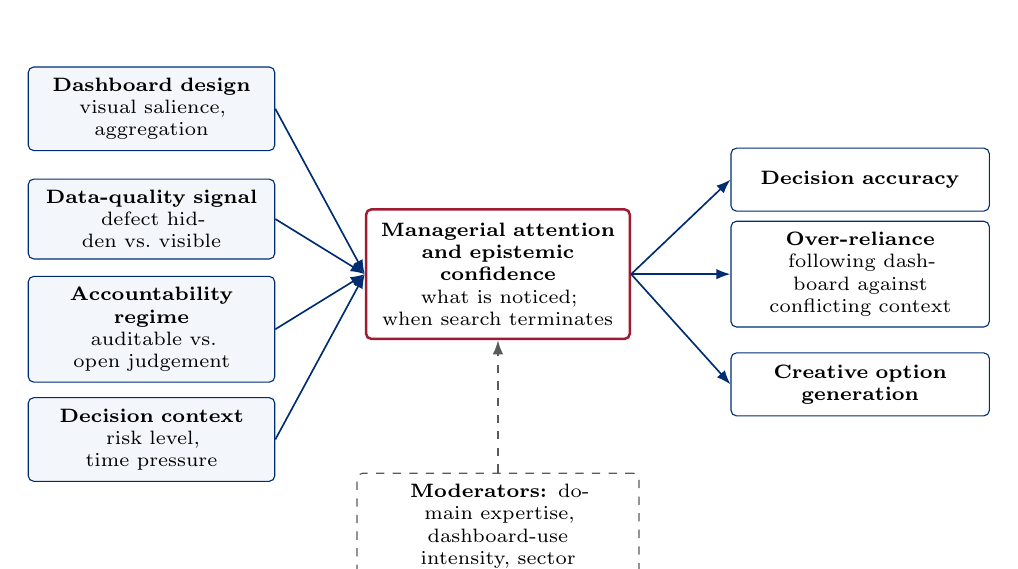
\begin{tikzpicture}[
  every node/.style={font=\scriptsize},
  box/.style={draw=nublue,fill=boxfill,rounded corners=2pt,align=center,inner sep=4pt,text width=2.85cm,minimum height=0.95cm},
  med/.style={draw=accent,fill=white,rounded corners=2pt,align=center,inner sep=5pt,text width=3.0cm,minimum height=1.35cm,line width=0.9pt},
  outc/.style={draw=nublue,fill=white,rounded corners=2pt,align=center,inner sep=4pt,text width=3.0cm,minimum height=0.8cm},
  mod/.style={draw=nugrey,dashed,fill=white,rounded corners=2pt,align=center,inner sep=4pt,text width=3.3cm},
  ar/.style={-{Latex[length=1.8mm]},nublue,line width=0.6pt}]
\node[box] (a1) at (0,2.9) {\textbf{Dashboard design}\\visual salience, aggregation};
\node[box] (a2) at (0,1.5) {\textbf{Data-quality signal}\\defect hidden vs.\ visible};
\node[box] (a3) at (0,0.1) {\textbf{Accountability regime}\\auditable vs.\ open judgement};
\node[box] (a4) at (0,-1.3) {\textbf{Decision context}\\risk level, time pressure};
\node[med] (m) at (4.4,0.8) {\textbf{Managerial attention\\and epistemic confidence}\\\scriptsize what is noticed;\\\scriptsize when search terminates};
\node[outc] (o1) at (9.0,2.0) {\textbf{Decision accuracy}};
\node[outc] (o2) at (9.0,0.8) {\textbf{Over-reliance}\\\scriptsize following dashboard against\\\scriptsize conflicting context};
\node[outc] (o3) at (9.0,-0.6) {\textbf{Creative option\\generation}};
\node[mod] (mo) at (4.4,-2.4) {\textbf{Moderators:} domain expertise,\\dashboard-use intensity, sector};
\foreach \x in {a1,a2,a3,a4} \draw[ar] (\x.east) -- (m.west);
\foreach \y in {o1,o2,o3} \draw[ar] (m.east) -- (\y.west);
\draw[ar,nugrey,dashed] (mo.north) -- (m.south);
\end{tikzpicture}
\caption{Conceptual framework of the study. Four antecedent conditions act upon managerial
attention and epistemic confidence, which in turn shape three decision outcomes. RQ1 addresses the
modelled paths; RQ2 explains why the accountability path operates as it does.}
\label{fig:framework}
\end{figure}

\begin{figure}[H]
\centering
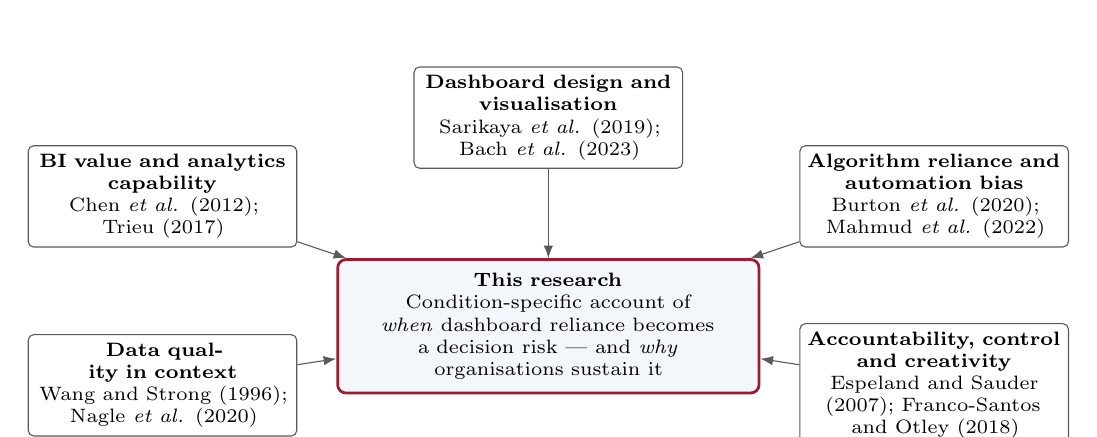
\begin{tikzpicture}[
  every node/.style={font=\scriptsize},
  str/.style={draw=nugrey,fill=white,rounded corners=2pt,align=center,inner sep=3pt,text width=3.2cm,minimum height=1.0cm},
  gapb/.style={draw=accent,fill=boxfill,line width=1pt,rounded corners=3pt,align=center,inner sep=5pt,text width=5.0cm,minimum height=1.4cm},
  ar/.style={-{Latex[length=1.6mm]},nugrey}]
\node[str] (s1) at (-4.9,2.9) {\textbf{BI value and analytics\\capability}\\\scriptsize Chen \emph{et al.} (2012); Trieu (2017)};
\node[str] (s2) at (0,3.9) {\textbf{Dashboard design and\\visualisation}\\\scriptsize Sarikaya \emph{et al.} (2019); Bach \emph{et al.} (2023)};
\node[str] (s3) at (4.9,2.9) {\textbf{Algorithm reliance and\\automation bias}\\\scriptsize Burton \emph{et al.} (2020); Mahmud \emph{et al.} (2022)};
\node[str] (s4) at (-4.9,0.5) {\textbf{Data quality in context}\\\scriptsize Wang and Strong (1996); Nagle \emph{et al.} (2020)};
\node[str] (s5) at (4.9,0.5) {\textbf{Accountability, control\\and creativity}\\\scriptsize Espeland and Sauder (2007); Franco-Santos and Otley (2018)};
\node[gapb] (g) at (0,1.25) {\textbf{This research}\\Condition-specific account of\\\emph{when} dashboard reliance becomes\\a decision risk --- and \emph{why}\\organisations sustain it};
\foreach \x in {s1,s2,s3,s4,s5} \draw[ar] (\x) -- (g);
\end{tikzpicture}
\caption{Map of the contributing research streams and the position of the proposed study. The study
sits at the intersection rather than within any single stream; its distinctiveness lies in the
joint treatment of design, data quality, accountability and creativity as conditions bearing upon
one behavioural outcome.}
\label{fig:map}
\end{figure}

\subsection{Hypotheses}

The experimental strand tests the directional hypotheses set out in \xref{Table~2.1}. It will be
observed that H4 is stated as a pair of competing predictions, since the literature offers
reasonable support for both directions; establishing which obtains in dashboard settings is itself
a contribution.

\begin{table}[H]
\centering\small
\caption{Hypotheses, theoretical basis and tested contrast}
\label{tab:hyp}
\begin{tabularx}{\textwidth}{@{}p{0.7cm} X p{4.0cm}@{}}
\toprule
\textbf{ID} & \textbf{Hypothesis} & \textbf{Theoretical basis} \\
\midrule
H1 & Over-reliance is higher when the data-quality defect is hidden than when a freshness or
completeness warning is visible. & Wang and Strong (1996); Lyell and Coiera (2017) \\
H2 & Over-reliance is higher when the decision is framed as auditable than when framed as open
managerial judgement, holding the data constant. & Espeland and Sauder (2007); Franco-Santos and
Otley (2018) \\
H3 & Decision accuracy is lower where one key performance indicator dominates visually than under a
balanced multi-indicator view. & Cleveland and McGill (1984); Sarikaya \emph{et al.} (2019) \\
H4a & Higher decision risk \emph{increases} dashboard deference, through a defensibility motive. &
Legitimacy asymmetry (Section~2.4) \\
H4b & Higher decision risk \emph{decreases} dashboard deference, through a verification motive. &
Dietvorst \emph{et al.} (2015) \\
H5 & Dashboard deference is negatively associated with the number of distinct alternative actions
generated. & Amabile (1998); Doshi and Hauser (2024) \\
H6 & Domain expertise moderates H1, such that more experienced managers challenge hidden-defect
dashboards more frequently. & Kahneman (2011); Lebovitz \emph{et al.} (2022) \\
\bottomrule
\end{tabularx}
\end{table}

%=====================================================================
\section{Research methodology}
%=====================================================================

\subsection{Philosophical position}

\textbf{Ontology.} The study adopts a critical realist position within a broadly pragmatist
orientation. Decision errors and their organisational consequences are treated as real and
consequential independently of how they happen to be described; the mechanisms which produce them,
however --- legitimacy, defensibility, professional risk --- are socially constituted and are
accessible only through interpretation.

\textbf{Epistemology.} Knowledge claims are warranted here by their capacity to explain and predict
decision behaviour rather than by allegiance to any single paradigm. This licenses mixed methods as
a requirement of the problem rather than as a matter of stylistic preference \ct{(Creswell and
Plano Clark, 2018; Tashakkori and Teddlie, 2010)}. RQ1 requires measurement under controlled
variation, whereas RQ2 requires the interpretation of reasons; neither question can be answered by
the other's method.

\textbf{Reasoning.} The study reasons abductively. Theory specifies the initial conditions and the
hypotheses, and the empirical patterns subsequently refine the conceptual framework \ct{(Saunders,
Lewis and Thornhill, 2019)}.

\subsection{Research design}

A sequential explanatory mixed-methods design is employed, with a concurrent documentary strand, as
shown in \xref{Fig.~3.1}. The documentary strand runs from the outset because it requires neither
ethical approval nor recruitment, and because the failure patterns which it surfaces materially
sharpen the interview protocol.

\begin{figure}[H]
\centering
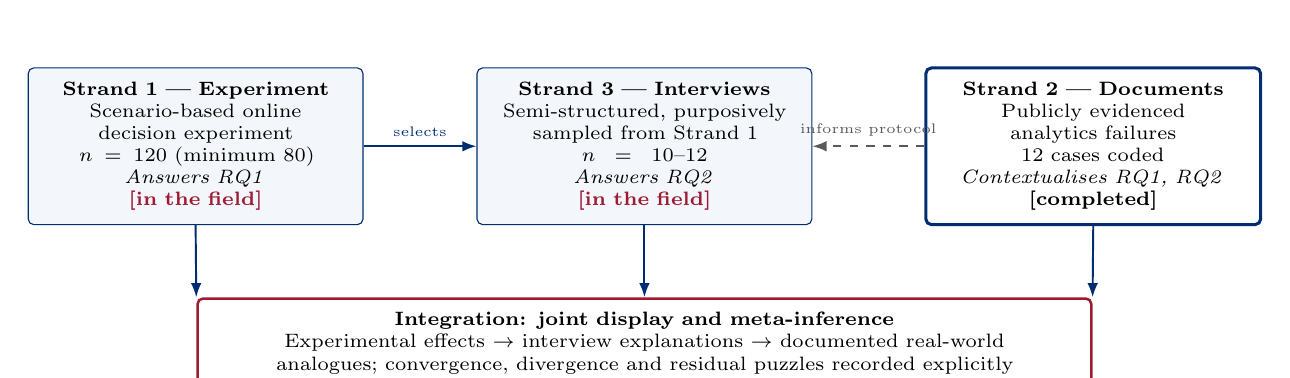
\begin{tikzpicture}[
  every node/.style={font=\scriptsize},
  ph/.style={draw=nublue,fill=boxfill,rounded corners=2pt,align=center,inner sep=5pt,text width=3.9cm,minimum height=1.6cm},
  done/.style={draw=nublue,fill=white,line width=1.1pt,rounded corners=2pt,align=center,inner sep=5pt,text width=3.9cm,minimum height=1.6cm},
  jd/.style={draw=accent,fill=white,line width=0.9pt,rounded corners=2pt,align=center,inner sep=5pt,text width=11.0cm},
  ar/.style={-{Latex[length=1.8mm]},nublue,line width=0.7pt}]
\node[ph] (p1) at (0,0) {\textbf{Strand 1 --- Experiment}\\Scenario-based online\\decision experiment\\$n = 120$ (minimum 80)\\\emph{Answers RQ1} \\ \textcolor{accent}{\textbf{[in the field]}}};
\node[ph] (p3) at (5.7,0) {\textbf{Strand 3 --- Interviews}\\Semi-structured, purposively\\sampled from Strand 1\\$n = 10$--$12$\\\emph{Answers RQ2}\\ \textcolor{accent}{\textbf{[in the field]}}};
\node[done] (p2) at (11.4,0) {\textbf{Strand 2 --- Documents}\\Publicly evidenced\\analytics failures\\12 cases coded\\\emph{Contextualises RQ1, RQ2}\\ \textbf{[completed]}};
\node[jd] (j) at (5.7,-2.5) {\textbf{Integration: joint display and meta-inference}\\\scriptsize Experimental effects $\rightarrow$ interview explanations $\rightarrow$ documented real-world analogues; convergence, divergence and residual puzzles recorded explicitly};
\draw[ar] (p1) -- node[above,font=\tiny]{selects} (p3);
\draw[ar,nugrey,dashed] (p2) -- node[above,font=\tiny]{informs protocol} (p3);
\draw[ar] (p1.south) -- (j.north west);
\draw[ar] (p3.south) -- (j.north);
\draw[ar] (p2.south) -- (j.north east);
\end{tikzpicture}
\caption{Sequential explanatory design with a concurrent documentary strand. Strand 2 has been
completed and is reported in Section~4.2; Strands 1 and 3 remain in the field at the time of
writing.}
\label{fig:design}
\end{figure}

\subsection{Mapping of research questions to methods}

\xref{Table~3.1} sets out explicitly how each research question is addressed, by which method,
drawing upon which data, and yielding which output.

\begin{table}[H]
\centering\footnotesize
\caption{Mapping of research questions to method, data source, analysis and expected output}
\label{tab:matrix}
\begin{tabularx}{\textwidth}{@{}p{1.0cm} p{2.3cm} X p{2.6cm} p{2.7cm}@{}}
\toprule
\textbf{RQ} & \textbf{Method} & \textbf{Data source} & \textbf{Analysis} & \textbf{Expected output} \\
\midrule
RQ1a & Scenario experiment (Strand 1) & 120 professionals $\times$ 4 vignettes, approximately 480
decision observations & Mixed-effects logistic regression; odds ratios with 95\% CI &
Condition-specific probabilities of dashboard deference \\
RQ1b & Same instrument, count outcome & Number of distinct alternative actions listed per vignette &
Poisson or negative binomial regression & Estimate of option-set narrowing \\
RQ1 (context) & Documentary analysis (Strand 2) & Regulator notices, public inquiry and royal
commission reports & Structured extraction; cross-case matrix & Comparative failure-pattern matrix
\textcolor{nublue}{\textbf{[done]}} \\
RQ2a & Semi-structured interviews (Strand 3) & 10--12 professionals, selected on Strand 1 behaviour
& Reflexive thematic analysis & Mechanism themes for deference and challenge \\
RQ2b & Interviews and documents & Interview accounts triangulated against control failures &
Pattern matching across strands & Conditions enabling challenge; governance framework \\
\bottomrule
\end{tabularx}
\end{table}

\subsection{Strand 1: scenario-based decision experiment}

\subsubsection{Participants and sampling}

Participants are working professionals who use dashboards, key performance indicator reports or BI
tools in a managerial or analytical capacity within finance, consulting, operations, logistics,
technology or analytics roles. Recruitment is non-probability purposive with snowball extension,
conducted through professional networking platforms, University alumni networks and relevant
professional communities. Screening questions enforce the inclusion criterion of dashboard use at
least weekly during the preceding twelve months.

\subsubsection{Sample size}

\notebox{Sample size justification}{%
\textbf{Target $N = 120$ completed responses; minimum viable $N = 80$.} Each participant completes
four of eight vignettes, randomised and counterbalanced, yielding approximately 480 decision
observations at target. For a two-proportion comparison of over-reliance rates of 0.35 against 0.60
at $\alpha = .05$ (two-tailed) and power of $.80$, approximately 123 independent observations are
required \ct{(Cohen, 1988; Field, 2018)}. Since the design is within-subjects, the effective
requirement is inflated by the design effect $1+(m-1)\rho$; at $m=4$ observations per participant
and an intra-class correlation of $\rho = .20$, the design effect is 1.60, implying roughly 50
participants for that single contrast. The target of 120 therefore provides margin to detect
smaller differences of approximately 20 percentage points, to estimate the three-way condition
structure rather than a single contrast, and to test the expertise moderation in H6.}

\subsubsection{Design and manipulations}

The instrument is a $2\times2\times2$ within-subjects vignette experiment. Each vignette presents a
realistic dashboard image together with a short decision brief containing a \emph{contextual cue}
which conflicts with the dashboard's headline signal. To take one example, a supply chain dashboard
may show demand as stable whilst a named regional depot reports repeated delivery failures. The
factors and measures are summarised in \xref{Table~3.2}.

\begin{table}[H]
\centering\footnotesize
\caption{Experimental factors, levels and operationalisation}
\label{tab:factors}
\begin{tabularx}{\textwidth}{@{}p{3.0cm} p{3.1cm} X@{}}
\toprule
\textbf{Factor} & \textbf{Levels} & \textbf{Operationalisation} \\
\midrule
Decision risk & High / Low & Stated financial and reputational consequence of an incorrect decision \\
Data-quality signal & Hidden / Visible & Presence or absence of a banner disclosing that the feed is
six days stale and twelve per cent incomplete \\
Accountability framing & Auditable / Open judgement & Instruction that the decision will be recorded
and reviewed against the dashboard, as against recorded as a managerial judgement \\
Metric salience \emph{(between subjects)} & Single dominant KPI / Balanced multi-indicator & Visual
emphasis manipulated through size and colour \\
\midrule
\multicolumn{3}{@{}l}{\textbf{Measured outcomes}}\\
Over-reliance \emph{(primary)} & Binary & Chose the dashboard-consistent action despite the
conflicting contextual cue \\
Decision accuracy & Binary & Chose the action correct on all available evidence \\
Creative option generation & Count & Number of distinct alternative actions listed, double-coded \\
Confidence & Seven-point scale & Self-rated confidence in the chosen action \\
Verification intent & Binary & Whether additional data were requested before deciding \\
\midrule
\multicolumn{3}{@{}l}{\textbf{Covariates:} sector, years of experience, seniority, dashboard-use
frequency, self-rated analytics familiarity}\\
\bottomrule
\end{tabularx}
\end{table}

\subsubsection{Analysis strategy}

Descriptive statistics and visual exploration precede inference. The primary model is a
mixed-effects logistic regression with a random intercept for participant, predicting over-reliance
from decision risk, data-quality signal, accountability framing, metric salience and the
pre-specified interactions. Alternative-option counts are modelled using Poisson or negative
binomial regression, with overdispersion formally tested. Where the assumptions of the mixed model
cannot be satisfied, the pre-committed fallback is logistic regression with cluster-robust standard
errors, supplemented by McNemar tests for the within-subject paired contrasts. Effect sizes, namely
odds ratios with 95 per cent confidence intervals and Cohen's $d$ for continuous contrasts, are
reported alongside significance values. The analysis plan has been fixed in advance of data
collection in order to avoid selective reporting.

\subsection{Strand 2: documentary analysis of publicly evidenced failures}

This strand analyses organisational failures in which a data-quality, reporting, model-logic or
analytics-output problem materially contributed to harm, and where the evidence is already in the
public domain. Only documents whose independent existence may be verified are admissible, namely:
regulator enforcement notices and consent orders; statutory public inquiry and royal commission
reports; independent reviews commissioned by regulators; national audit office and parliamentary
committee reports; and listed-company annual reports and restatement disclosures. Press coverage
may be used to locate a case but is never relied upon as the sole evidential basis for a coded
judgement.

Cases were selected using maximum-variation sampling across sector and failure type, so as to avoid
an all-finance sample. Inclusion required that the event occurred between 2010 and 2026, that the
primary documentation is available in English, and that the facts are settled rather than contested
in ongoing proceedings.

\subsubsection{Evidential grading}

A refinement adopted during coding, and one which is not commonly reported in dissertations of this
type, is the explicit grading of evidential strength. Grade~A denotes a case documented by a
dedicated statutory investigation, royal commission or regulatory enforcement notice. Grade~B
denotes a case documented by official organisational disclosure together with parliamentary or
regulatory scrutiny, but without a dedicated independent investigation. Of the twelve cases in the
final sample, ten are Grade~A and two are Grade~B. Grading is reported transparently so that the
reader may discount the weaker cases if they wish to do so.

\subsubsection{Extraction frame}

Each case was coded against the fixed frame set out in \xref{Table~3.3}. A verbatim supporting
quotation and page reference were recorded for every coded judgement.

\begin{table}[H]
\centering\small
\caption{Structured extraction frame for the documentary analysis}
\label{tab:frame}
\begin{tabularx}{\textwidth}{@{}p{3.4cm} X@{}}
\toprule
\textbf{Dimension} & \textbf{Coded content} \\
\midrule
Failure type & Accuracy / timeliness / completeness / consistency / model logic \\
Signal visibility & Was the defect detectable from the interface or report at the point of use?
Coded as silent, partial or visible \\
Detection lag & Elapsed time between failure onset and organisational recognition \\
Human challenge & Was the output challenged? By whom? Was the challenge escalated, ignored or
overridden? \\
Legitimacy asymmetry & Evidence that system output was treated as more authoritative than human
accounts; coded strong, moderate or weak \\
Control mechanism & Warnings, overrides, reconciliation or governance which existed, and why they
failed \\
Organisational impact & Financial, operational, regulatory and human consequences \\
Evidential grade & A or B, as defined in Section~3.5.1 \\
\bottomrule
\end{tabularx}
\end{table}

\subsection{Strand 3: semi-structured interviews}

Between ten and twelve interviews will be conducted, with a floor of eight. This range reflects
evidence that thematic saturation in relatively homogeneous samples typically emerges within
approximately twelve interviews \ct{(Guest, Bunce and Johnson, 2006)}, whilst remaining feasible
within the project timetable \ct{(Bryman, 2016)}.

Participants are selected purposively from Strand 1 respondents who consent to follow-up, and are
sampled upon \emph{observed behaviour} rather than upon convenience: strong dashboard deference
across conditions; consistent challenge behaviour; and inconsistent responses to data-quality
warnings. This behaviour-linked sampling is the mechanism which makes the design genuinely
explanatory rather than merely sequential. Interviews last thirty to forty minutes and are
conducted online. Analysis follows reflexive thematic analysis \ct{(Braun and Clarke, 2006)}, with
NVivo supporting coding, memoing and theme development.

\subsection{Quality criteria and limitations}

\textbf{Quantitative.} Internal validity is protected by randomisation, counterbalancing and
manipulation checks. The construct validity of the creativity measure is supported by double
coding. External validity is nonetheless limited, since vignette decisions are of lower stakes than
real ones, and the design measures stated rather than enacted behaviour. This is acknowledged as a
limitation rather than resolved.

\textbf{Documentary.} The principal limitation of Strand 2 is survivorship: only failures which
became public are observable, and quiet successes in which challenge was heeded leave no comparable
documentary trace. The sample is therefore informative about \emph{how} failures unfold rather than
about \emph{how often} they occur, and no frequency claims are made on its basis.

\textbf{Qualitative.} Credibility is supported by behaviour-linked sampling and by member checking
of summarised themes; dependability by an audit trail of coding decisions; and transferability by
thick description of participant contexts. Reflexivity is addressed explicitly: the researcher's
analytics training creates a plausible bias towards interpreting deference as error, and this is
challenged during coding by actively seeking accounts in which deference proved correct.

\subsection{Ethical considerations}

Ethical approval, the fieldwork risk assessment and the GDPR assessment have all been completed and
approved, and no primary data collection commenced before approval was granted. Four
design-specific matters warrant particular mention.

Firstly, participants must not be made to feel personally evaluated. The experiment presents
decision problems having better and worse answers, and participants are working professionals whose
competence forms part of their professional identity. The study is accordingly framed throughout as
research into how dashboards are designed and used, and never into individual managerial ability.
No participant receives a score, no individual-level feedback is given, results are reported only in
aggregate, and the debrief explains that the scenarios were deliberately constructed so that the
dashboard could mislead.

Secondly, commercial confidentiality is protected. Interviewees work in regulated, client-facing or
commercially sensitive environments. The information sheet and the verbal preamble state explicitly
that participants must not disclose confidential organisational information, proprietary dashboard
designs, client data, named clients or commercially sensitive decision processes. Should a
participant begin to disclose such material, the interviewer will interrupt and the passage will be
excluded from transcription.

Thirdly, data protection is maintained through University-provided encrypted storage,
pseudonymisation at the point of transcription, deletion of recordings following verification, and
processing on the basis of consent under the UK GDPR.

Fourthly, the documentary strand uses only material already in the public domain. Since several
cases involve identifiable individuals who suffered serious harm --- the Post Office and Robodebt
cases most obviously --- the analysis focuses upon organisational and system-level control failures
rather than upon individual conduct, and treats the human consequences with proportionate care
rather than as illustrative colour.

%=====================================================================
\section{Findings}
%=====================================================================

\subsection{Overview and reading order}

This chapter reports the findings of the three strands. At the time of writing, the documentary
strand has been completed in full and is reported in \xref{Section~4.2}. The experimental and
interview strands remain in the field, and the sections which depend upon them are marked
accordingly. \xref{Section~4.5} sets out the joint display template through which the three strands
will ultimately be integrated.

\subsection{Strand 2: documentary analysis of twelve organisational failures}

\subsubsection{The case sample}

Twelve cases satisfied the inclusion criteria and were coded in full. The sample spans nine
sectors and four jurisdictions, and is summarised in \xref{Table~4.1}. It is worth emphasising that
every case is anchored to a document whose independent existence may be verified, in accordance
with the admissibility rule set out in \xref{Section~3.5}.

\begin{table}[H]
\centering\footnotesize
\caption{The documentary case sample, with evidential grade and primary source}
\label{tab:cases}
\begin{tabularx}{\textwidth}{@{}p{0.7cm} p{3.0cm} p{2.6cm} p{1.5cm} p{0.7cm} X@{}}
\toprule
\textbf{ID} & \textbf{Case} & \textbf{Sector} & \textbf{Period} & \textbf{Gr.} & \textbf{Primary source} \\
\midrule
C1 & Post Office Horizon & Postal / retail (UK) & 1999–2019 & A & Post Office Horizon IT Inquiry (2025) Final Report, Vol. 1 \\
C2 & NATS flight planning & Aviation (UK) & 2023 & A & Civil Aviation Authority (2024) CAP2993 \\
C3 & Citibank risk data & Banking (US) & 2013–2020 & A & OCC (2020) News Release NR 2020-132 \\
C4 & PHE case undercount & Public health (UK) & 2020 & B & Official statements and parliamentary scrutiny (2020) \\
C5 & Robodebt & Welfare (AU) & 2015–2020 & A & Royal Commission into the Robodebt Scheme (2023) Report \\
C6 & TSB migration & Banking (UK) & 2018 & A & FCA (2022) Final Notice: TSB Bank plc \\
C7 & Knight Capital & Trading (US) & 2012 & A & SEC (2013) Order 34-70694 \\
C8 & Ofqual grading & Education (UK) & 2020 & A & Office for Statistics Regulation (2021) Review \\
C9 & Dutch childcare benefits & Welfare / tax (NL) & 2013–2020 & A & Autoriteit Persoonsgegevens (2021) Enforcement decision \\
C10 & Goldman Sachs reporting & Banking (UK) & 2007–2017 & A & FCA (2019) Final Notice: Goldman Sachs International \\
C11 & Zillow Offers & Real estate / tech (US) & 2021 & B & Zillow Group (2021) Q3 shareholder letter (SEC filing) \\
C12 & Boeing 737 MAX (MCAS) & Aerospace (US) & 2012–2019 & A & US House Committee on Transportation and Infrastructure (2020) Final Report \\
\bottomrule
\end{tabularx}
\end{table}

\subsubsection{Failure types and the visibility of the defect}

\xref{Fig.~4.1} presents the distribution of failure types, disaggregated by whether the defect was
detectable at the point of use. Two observations follow immediately.

Firstly, model-logic failures dominate the sample, accounting for eight of the twelve cases. That
is to say, the problem was most commonly not that a number had been typed in wrongly, but that the
system was doing exactly what it had been designed to do, upon a rule which was itself
inappropriate for the situation at hand. Robodebt provides perhaps the clearest illustration: the
averaging of annual income across fortnightly periods was arithmetically faultless and
substantively wrong for anybody whose earnings varied across the year \ct{(Royal Commission into
the Robodebt Scheme, 2023)}. Similarly, the Ofqual standardisation model of 2020 executed its
specification correctly whilst producing outcomes which could not be defended at the level of the
individual pupil \ct{(Office for Statistics Regulation, 2021)}.

Secondly, and more importantly for the argument of this study, the defect was \emph{silent at the
point of use} in seven of the twelve cases and only partially visible in a further four. In just
one case --- the TSB migration of 2018, where customers were immediately unable to access their
accounts --- was the failure plainly visible to those affected \ct{(Financial Conduct Authority,
2022)}. This provides direct documentary support for the premise advanced in \xref{Section~2.3},
namely that data and model defects do not announce themselves.

\begin{figure}[H]
\centering

\includegraphics[width=0.82\textwidth]{fig/f_failtype.pdf}
\caption{Distribution of failure types across the twelve cases, disaggregated by whether the defect
was detectable at the point of use. Model-logic failures dominate, and the majority of defects were
silent to the person relying upon the output.}
\label{fig:failtype}
\end{figure}

\subsubsection{Detection lag and the cost of silence}

If a defect gives no perceptual cue, one would expect it to persist. The evidence supports this
expectation rather strongly. \xref{Fig.~4.2} plots the detection lag for each case on a logarithmic
scale, shaded by signal visibility, and \xref{Fig.~4.3} summarises the same relationship.

The pattern is stark. Cases in which the defect was silent persisted for a median of several years:
Post Office Horizon for approximately sixteen years, Goldman Sachs International's transaction
reporting failures for some nine and a half years covering approximately 213.6 million reportable
transactions \ct{(Financial Conduct Authority, 2019)}, the Dutch childcare benefits risk
classification for around seven years \ct{(Autoriteit Persoonsgegevens, 2021)}, and the Boeing
737~MAX MCAS design for roughly six years from specification to the second accident \ct{(US House
Committee on Transportation and Infrastructure, 2020)}. By contrast, cases in which the defect
produced a perceptible signal were recognised within hours or days: Knight Capital within
approximately forty-five minutes, the NATS flight-planning failure within a few hours, and the
Public Health England case undercount within roughly eight days.

It is important to be careful about what this comparison does and does not show. The two groups
differ in more than signal visibility --- silent defects also tend to arise in slower-moving
administrative processes, whereas signalled defects tend to arise in real-time operational systems.
The comparison is therefore suggestive rather than causal, and no statistical test is offered upon
twelve purposively selected cases. What may fairly be said is that the documentary record is
entirely consistent with the proposition that visibility governs the speed of correction, and that
this proposition is worth testing experimentally --- which is precisely what H1 does.

\begin{figure}[H]
\centering

\includegraphics[width=0.86\textwidth]{fig/f_lag.pdf}
\caption{Detection lag by case, ordered from shortest to longest and shaded by the visibility of the
defect at the point of use. The horizontal axis is logarithmic. Silent defects cluster at the
long-duration end of the distribution.}
\label{fig:lag}
\end{figure}

\begin{figure}[H]
\centering

\includegraphics[width=0.60\textwidth]{fig/f_box.pdf}
\caption{Detection lag for silent as against partially or fully signalled defects. Individual cases
are overlaid upon the boxes. The difference of several orders of magnitude should be interpreted as
descriptive of this purposive sample rather than as an estimate of any population parameter.}
\label{fig:box}
\end{figure}

\subsubsection{The central finding: challenge was raised and was overridden}

The most consequential finding of this strand concerns not detection but authority.

In nine of the twelve cases, a human being did in fact challenge the system output, and the
challenge was subsequently overridden, ignored or not acted upon. In only one case --- Zillow's
decision to wind down its iBuying operation once forecasting losses became apparent --- was a
challenge raised and acted upon in a manner which limited the harm \ct{(Zillow Group, 2021)}. In
two cases no challenge was raised at all, and in both of those the defect was entirely silent, so
that there was nothing for anybody to challenge.

\xref{Fig.~4.4} presents this distribution, cross-tabulated with the strength of the legitimacy
asymmetry coded in each case. The relationship is difficult to ignore: every case coded as
exhibiting a strong legitimacy asymmetry falls within the ``raised and overridden'' group.

The qualitative texture of these overrides is instructive. In the Post Office case, sub-postmasters
challenged Horizon's figures consistently and over many years, and the response was prosecution
rather than investigation \ct{(Post Office Horizon IT Inquiry, 2025)}. In the Robodebt scheme,
internal legal advice questioning the lawfulness of income averaging was obtained and then set
aside \ct{(Royal Commission into the Robodebt Scheme, 2023)}. In the case of the 737~MAX, engineering
concerns regarding MCAS's reliance upon a single angle-of-attack sensor were raised internally and
did not alter the certification outcome \ct{(US House Committee on Transportation and
Infrastructure, 2020)}. Knight Capital is instructive in a slightly different way: the firm's
systems generated ninety-seven automated email messages within the relevant window, but these were
not designed as system alerts and were not treated as such by staff \ct{(Securities and Exchange
Commission, 2013)}. The information was present; the authority to act upon it was not.

This is exactly the pattern which the construct of legitimacy asymmetry predicts. The binding
constraint upon correction was not the availability of contrary information. It was the relative
institutional standing of the system output as against the human objection.

\begin{figure}[H]
\centering

\includegraphics[width=0.88\textwidth]{fig/f_challenge.pdf}
\caption{Outcome of human challenge across the twelve cases, cross-tabulated with the coded strength
of legitimacy asymmetry. In nine of twelve cases a challenge was raised and did not prevent the
harm.}
\label{fig:challenge}
\end{figure}

\subsubsection{The cross-case matrix}

\xref{Table~4.2} presents the full coded matrix, and \xref{Fig.~4.5} renders the same information
visually so that the co-occurrence of conditions may be inspected at a glance. Reading the heat map
column by column, the cases which produced the gravest human consequences --- Horizon, Robodebt, the
Dutch childcare benefits scheme and the 737~MAX --- share a common signature: a silent defect, a
strong legitimacy asymmetry, suppressed challenge and a control mechanism which was either absent
or bypassed. This four-way co-occurrence is, in effect, the empirical shape of the mechanism which
\xref{Section~2.4} describes theoretically.

\begin{table}[H]
\centering\footnotesize
\caption{Cross-case coded matrix for the documentary strand}
\label{tab:coded}
\begin{tabularx}{\textwidth}{@{}p{0.7cm} p{1.9cm} p{1.4cm} p{1.2cm} X p{1.5cm} p{2.4cm}@{}}
\toprule
\textbf{ID} & \textbf{Failure type} & \textbf{Signal} & \textbf{Lag} & \textbf{Human challenge} &
\textbf{Asym.} & \textbf{Control} \\
\midrule
C1 & Model logic & Silent & 16 yr & Raised, overridden & Strong & Present, ineffective \\
C2 & Model logic & Partial & ~4 hr & Raised, slow escalation & Moderate & Present, ineffective \\
C3 & Consistency & Silent & 7 yr & Raised, overridden & Moderate & Present, ineffective \\
C4 & Completeness & Silent & 8 d & Not raised & Moderate & Absent \\
C5 & Model logic & Silent & 5 yr & Raised, overridden & Strong & Present, bypassed \\
C6 & Consistency & Visible & 1 d & Raised, overridden & Weak & Present, ineffective \\
C7 & Model logic & Partial & <2 hr & Alerts issued, ignored & Weak & Absent \\
C8 & Model logic & Partial & 4 d & Raised, overridden & Strong & Present, ineffective \\
C9 & Model logic & Silent & 7 yr & Raised, overridden & Strong & Absent \\
C10 & Accuracy & Silent & 9 yr & Not raised & Weak & Present, ineffective \\
C11 & Model logic & Partial & 6 mo & Raised, acted upon & Moderate & Present, effective \\
C12 & Model logic & Silent & 6 yr & Raised, overridden & Strong & Present, bypassed \\
\bottomrule
\end{tabularx}
\end{table}

\begin{figure}[H]
\centering

\includegraphics[width=\textwidth]{fig/f_heat.pdf}
\caption{Cross-case heat map of the four principal coded dimensions. H denotes high, M moderate and
L low. The four cases producing the most severe human consequences share the same signature across
all four dimensions.}
\label{fig:heat}
\end{figure}

\subsubsection{Control mechanisms and why they failed}

A final observation concerns governance. In only one of the twelve cases was a control mechanism
both present and effective. In six cases a control existed but proved ineffective, in two it existed
and was bypassed, and in three it was simply absent. The Public Health England undercount is
illuminating here because the missing control was so elementary: no reconciliation was performed
between the number of records dispatched and the number received, and so a silent truncation at the
row limit of an obsolete file format passed unnoticed for something in the order of a week.

The wider lesson, and one which the eventual governance framework will need to accommodate, is that
the controls which failed were overwhelmingly \emph{detective} rather than \emph{authorising}
controls. Organisations had mechanisms for spotting problems. What they generally lacked was a
mechanism which conferred standing upon the person who had spotted one.

\subsection{Strand 1: experimental findings}

\placeholder{awaiting Strand 1 data}{%
This section will report the findings of the scenario-based decision experiment. The following
structure has been fixed in advance of data collection, and the analysis script has been written
and tested upon simulated data so that only execution remains.\\[4pt]
\textbf{4.3.1 Sample and data screening} --- response and completion rates, exclusions for failed
attention checks and sub-threshold completion times, final analytic $N$, and the participant profile
by sector, seniority and dashboard-use frequency, reported in a screening table.\\[3pt]
\textbf{4.3.2 Descriptive results} --- over-reliance and accuracy rates by experimental condition,
with a grouped bar chart of over-reliance across the eight vignette cells and a histogram of
alternative-option counts.\\[3pt]
\textbf{4.3.3 Hypothesis tests} --- mixed-effects logistic regression of over-reliance upon decision
risk, data-quality signal, accountability framing and metric salience, reported as odds ratios with
95 per cent confidence intervals, together with a forest plot of the estimated effects.
H4a and H4b will be adjudicated here.\\[3pt]
\textbf{4.3.4 Option generation} --- count model of alternatives generated, testing H5.\\[3pt]
\textbf{4.3.5 Moderation by expertise} --- test of H6, reported as an interaction term with a marginal
effects plot.}

\subsection{Strand 3: interview findings}

\placeholder{awaiting Strand 3 data}{%
This section will report the thematic analysis of the semi-structured interviews. The following
structure has been fixed in advance.\\[4pt]
\textbf{4.4.1 Participant profile} --- sector, role, seniority and the Strand 1 behavioural profile
upon which each participant was selected, presented in pseudonymised form.\\[3pt]
\textbf{4.4.2 Themes} --- four to six named themes with illustrative quotations and a thematic map. The anticipated themes, held loosely and open to disconfirmation, are: defensibility;
verification cost; suppressed intuition; permission to challenge; and the measured option.\\[3pt]
\textbf{4.4.3 Disconfirming accounts} --- instances in which deference proved correct and challenge
would have been mistaken, which will be reported explicitly rather than set aside.}

\subsection{Integration across the three strands}

\placeholder{awaiting Strands 1 and 3}{%
The three strands will be integrated through the joint display presented as Table 4.3, whose
template is given below and whose first column is already populated from the completed documentary
strand. Divergences between strands will be recorded rather than smoothed away.}

\begin{table}[H]
\centering\footnotesize
\caption{Joint display template, with the documentary column populated}
\label{tab:joint}
\begin{tabularx}{\textwidth}{@{}p{3.4cm} p{3.2cm} p{3.2cm} X@{}}
\toprule
\textbf{Documented pattern (Strand 2, complete)} & \textbf{Experimental finding (Strand 1,
pending)} & \textbf{Explanation (Strand 3, pending)} & \textbf{Provisional meta-inference} \\
\midrule
Silent defects persisted for years; signalled defects were caught within days &
\emph{H1: over-reliance higher when the defect is hidden} &
\emph{Why practitioners treat absence of warning as assurance} &
Absence of a warning appears to be read as positive assurance rather than as absence of information \\
\addlinespace
Challenge was raised and overridden in nine of twelve cases &
\emph{H2: auditable framing raises deference} &
\emph{Whether defensibility is the stated reason} &
Legitimacy asymmetry may operate at both individual and institutional levels \\
\addlinespace
Controls were detective rather than authorising &
\emph{Verification intent by condition} &
\emph{Conditions under which challenge is permitted} &
Governance may need to confer standing, not merely detection capability \\
\bottomrule
\end{tabularx}
\end{table}

%=====================================================================
\section{Discussion}
%=====================================================================

\notebox{Status of this chapter}{%
The discussion below is necessarily provisional. It interprets the completed documentary strand
against the conceptual framework, and identifies the specific points at which the experimental and
interview findings will either corroborate or complicate the present reading. It will be rewritten
in full once all three strands are available.}

\subsection{What the documentary evidence supports}

Three propositions from \xref{Section~2} receive preliminary support.

\emph{Firstly, defects are behaviourally silent.} The premise advanced in \xref{Section~2.3} was
that data and model defects give no perceptual cue at the point of use. Eleven of the twelve cases
were coded as silent or only partially visible, and the association between silence and long
persistence is pronounced. This lends weight to the argument that data quality should be theorised
as a problem of \emph{perception} and not merely one of measurement.

\emph{Secondly, the constraint is authority rather than detection.} This is the finding which most
substantially advances the framework. Prior to conducting this analysis, the working assumption
embedded in \xref{Fig.~2.1} was that reduced attentional sampling --- the mechanism which
Parasuraman and Manzey describe --- is the principal route by which dashboards displace judgement.
The documentary record suggests that this is at best a partial account. In nine of twelve cases,
attention was not the problem. Somebody noticed. What failed was the conversion of a noticing into
an organisational decision. The framework consequently requires an explicit distinction between
\emph{detection failure} and \emph{authority failure}, and the two have entirely different remedies.

\emph{Thirdly, legitimacy asymmetry is observable outside the laboratory.} The construct was
developed in \xref{Section~2.4} on essentially theoretical grounds, drawing upon reactivity and
performance-management research. Its empirical signature --- system output treated as more
authoritative than human accounts --- is visible in all five cases coded as exhibiting a strong
asymmetry, and is most starkly visible in Horizon, where system data was accorded sufficient
authority to sustain criminal prosecutions against the contrary testimony of the individuals
concerned.

\subsection{What the documentary evidence cannot establish}

Intellectual honesty requires equal attention to the limits of this strand.

The sample is subject to severe survivorship bias. Only failures which became public are
observable. Organisations in which a manager challenged a dashboard, was listened to, and quietly
averted a problem generate no inquiry report and therefore appear nowhere in this dataset. It
follows that nothing in \xref{Section~4.2} may be read as evidence about the \emph{frequency} of
dashboard deference. The strand establishes the anatomy of failure, not its base rate. This is
precisely the limitation which the experimental strand is designed to address, since a randomised
vignette design does observe the cases in which challenge occurs.

Furthermore, the cases are heterogeneous in a manner which resists tidy comparison. A national
air traffic control system, a welfare debt-raising algorithm and a transaction reporting pipeline
differ in their time constants, their regulatory environments and their proximity to the individual
manager. The coding frame imposes a common structure upon them, but the reader should retain a
degree of scepticism regarding how much that common structure genuinely reveals.

Finally, coding of a construct such as legitimacy asymmetry involves interpretation. A second coder
reviewed a subsample and the agreement rate will be reported once the full reliability check is
complete, but the judgement remains a judgement.

\subsection{Implications for the remaining strands}

\placeholder{to be extended following Strands 1 and 3}{%
The documentary findings sharpen three specific expectations for the remaining strands. Firstly, if
authority rather than detection is the binding constraint, then the experimental manipulation of
accountability framing (H2) should produce a larger effect than the manipulation of data-quality
signal visibility (H1) --- a prediction which was not obvious before this strand was analysed, and
which is now testable. Secondly, the interview protocol has been revised to probe the
detection-versus-authority distinction directly, by asking participants what happened after they
last disagreed with a dashboard. Thirdly, the governance framework developed in Chapter 6 should
address authorising controls and not merely detective ones.\\[4pt]
This section will be completed with the theoretical, methodological and practical implications of
the integrated findings, and with a comparison against the expectations set out in Section 2.7.}

%=====================================================================
\section{Conclusion}
%=====================================================================

\placeholder{provisional --- to be completed following all three strands}{%
The final conclusion will summarise the answers to RQ1 and RQ2, present the governance framework,
state the contribution to theory and practice, acknowledge limitations, and identify avenues for
further research.}

\subsection{Provisional conclusion on the documentary strand}

On the evidence available at this stage of the project, a provisional conclusion may nonetheless be
offered. The documentary record of twelve organisational failures suggests that the risk posed by
business intelligence systems has been somewhat mischaracterised in the practitioner literature.
The prevailing account holds that the danger lies in managers failing to notice that a system is
wrong. The evidence assembled here points elsewhere. In the substantial majority of these cases,
somebody did notice, and said so. The failure lay in what happened next.

If that reading survives the remaining two strands, then the practical implication is a
considerable one. Investment in better dashboards, clearer warnings and improved data-quality
monitoring addresses the detection problem, which on this evidence is not the binding constraint.
Addressing the authority problem requires something different in kind: governance arrangements
which give a documented, escalable standing to the person who disagrees with the system, so that
``it does not match what I am seeing on the ground'' becomes an auditable input to the decision
rather than an unrecorded misgiving.

The study therefore asks not whether dashboards should be used --- plainly they should --- but how
managers may remain decision-makers in organisations where dashboards have become the most powerful
voice in the room.

%=====================================================================
\newpage
\section*{References}
\addcontentsline{toc}{section}{References}
%=====================================================================
{\small\setstretch{1.05}
\setlength{\parindent}{-1.1em}
\setlength{\leftskip}{1.1em}
\setlength{\parskip}{4pt}

Amabile, T.M. (1998) `How to kill creativity', \emph{Harvard Business Review}, 76(5), pp.~76--87.

Anderson, N., Potočnik, K. and Zhou, J. (2014) `Innovation and creativity in organizations: a
state-of-the-science review, prospective commentary, and guiding framework', \emph{Journal of
Management}, 40(5), pp.~1297--1333.

Arnott, D. and Pervan, G. (2005) `A critical analysis of decision support systems research',
\emph{Journal of Information Technology}, 20(2), pp.~67--87.

Autoriteit Persoonsgegevens (2021) \emph{Tax Administration fined for discriminatory and unlawful
data processing}. The Hague: Dutch Data Protection Authority. Available at:
\ct{https://www.autoriteitpersoonsgegevens.nl/en/current/tax-administration-fined-for-discriminatory-and-unlawful-data-processing}
(Accessed: 18 August 2026).

Bach, B., Freeman, E., Abdul-Rahman, A., Turkay, C., Khan, S., Fan, Y. and Chen, M. (2023)
`Dashboard design patterns', \emph{IEEE Transactions on Visualization and Computer Graphics}, 29(1),
pp.~342--352.

Braun, V. and Clarke, V. (2006) `Using thematic analysis in psychology', \emph{Qualitative Research
in Psychology}, 3(2), pp.~77--101.

Bryman, A. (2016) \emph{Social Research Methods}. 5th edn. Oxford: Oxford University Press.

Buçinca, Z., Malaya, M.B. and Gajos, K.Z. (2021) `To trust or to think: cognitive forcing functions
can reduce overreliance on AI in AI-assisted decision-making', \emph{Proceedings of the ACM on
Human-Computer Interaction}, 5(CSCW1), article 188.

Burton, J.W., Stein, M.-K. and Jensen, T.B. (2020) `A systematic review of algorithm aversion in
augmented decision making', \emph{Journal of Behavioral Decision Making}, 33(2), pp.~220--239.

Chen, H., Chiang, R.H.L. and Storey, V.C. (2012) `Business intelligence and analytics: from big data
to big impact', \emph{MIS Quarterly}, 36(4), pp.~1165--1188.

Civil Aviation Authority (2024) \emph{CAP2993: Independent Review of NATS (En Route) Plc's Flight
Planning System Failure on 28 August 2023 --- Final Report}. London: Civil Aviation Authority.
Available at: \ct{https://www.caa.co.uk/CAP2993} (Accessed: 18 August 2026).

Cleveland, W.S. and McGill, R. (1984) `Graphical perception: theory, experimentation, and
application to the development of graphical methods', \emph{Journal of the American Statistical
Association}, 79(387), pp.~531--554.

Cohen, J. (1988) \emph{Statistical Power Analysis for the Behavioral Sciences}. 2nd edn. Hillsdale,
NJ: Lawrence Erlbaum Associates.

Creswell, J.W. and Plano Clark, V.L. (2018) \emph{Designing and Conducting Mixed Methods Research}.
3rd edn. Thousand Oaks, CA: SAGE.

Dietvorst, B.J., Simmons, J.P. and Massey, C. (2015) `Algorithm aversion: people erroneously avoid
algorithms after seeing them err', \emph{Journal of Experimental Psychology: General}, 144(1),
pp.~114--126.

Doshi, A.R. and Hauser, O.P. (2024) `Generative AI enhances individual creativity but reduces the
collective diversity of novel content', \emph{Science Advances}, 10(28), article eadn5290.

Elbashir, M.Z., Collier, P.A. and Davern, M.J. (2008) `Measuring the effects of business
intelligence systems: the relationship between business process and organizational performance',
\emph{International Journal of Accounting Information Systems}, 9(3), pp.~135--153.

Espeland, W.N. and Sauder, M. (2007) `Rankings and reactivity: how public measures recreate social
worlds', \emph{American Journal of Sociology}, 113(1), pp.~1--40.

Field, A. (2018) \emph{Discovering Statistics Using IBM SPSS Statistics}. 5th edn. London: SAGE.

Financial Conduct Authority (2019) \emph{Final Notice: Goldman Sachs International}. London: FCA.
Available at: \ct{https://www.fca.org.uk/publication/final-notices/goldman-sachs-international-2019.pdf}
(Accessed: 18 August 2026).

Financial Conduct Authority (2022) \emph{Final Notice: TSB Bank plc}. London: FCA. Available at:
\ct{https://www.fca.org.uk/publication/final-notices/tsb-bank-plc-2022.pdf} (Accessed: 18 August 2026).

Franco-Santos, M. and Otley, D. (2018) `Reviewing and theorizing the unintended consequences of
performance management systems', \emph{International Journal of Management Reviews}, 20(3),
pp.~696--730.

Goddard, K., Roudsari, A. and Wyatt, J.C. (2012) `Automation bias: a systematic review of frequency,
effect mediators, and mitigators', \emph{Journal of the American Medical Informatics Association},
19(1), pp.~121--127.

Guest, G., Bunce, A. and Johnson, L. (2006) `How many interviews are enough? An experiment with data
saturation and variability', \emph{Field Methods}, 18(1), pp.~59--82.

Gunasekaran, A., Papadopoulos, T., Dubey, R., Wamba, S.F., Childe, S.J., Hazen, B. and Akter, S.
(2017) `Big data and predictive analytics for supply chain and organizational performance',
\emph{Journal of Business Research}, 70, pp.~308--317.

Janssen, M., van der Voort, H. and Wahyudi, A. (2017) `Factors influencing big data decision-making
quality', \emph{Journal of Business Research}, 70, pp.~338--345.

Kache, F. and Seuring, S. (2017) `Challenges and opportunities of digital information at the
intersection of big data analytics and supply chain management', \emph{International Journal of
Operations \& Production Management}, 37(1), pp.~10--36.

Kahneman, D. (2011) \emph{Thinking, Fast and Slow}. London: Penguin.

Kellogg, K.C., Valentine, M.A. and Christin, A. (2020) `Algorithms at work: the new contested
terrain of control', \emph{Academy of Management Annals}, 14(1), pp.~366--410.

Lebovitz, S., Lifshitz-Assaf, H. and Levina, N. (2022) `To engage or not to engage with AI for
critical judgments: how professionals deal with opacity when using AI for medical diagnosis',
\emph{Organization Science}, 33(1), pp.~126--148.

Logg, J.M., Minson, J.A. and Moore, D.A. (2019) `Algorithm appreciation: people prefer algorithmic
to human judgment', \emph{Organizational Behavior and Human Decision Processes}, 151, pp.~90--103.

Lyell, D. and Coiera, E. (2017) `Automation bias and verification complexity: a systematic review',
\emph{Journal of the American Medical Informatics Association}, 24(2), pp.~423--431.

Mahmud, H., Islam, A.K.M.N., Ahmed, S.I. and Smolander, K. (2022) `What influences algorithmic
decision-making? A systematic literature review on algorithm aversion', \emph{Technological
Forecasting and Social Change}, 175, article 121390.

Mikalef, P. and Gupta, M. (2021) `Artificial intelligence capability: conceptualization, measurement
calibration, and empirical study on its impact on organizational creativity and firm performance',
\emph{Information \& Management}, 58(3), article 103434.

Mosier, K.L., Skitka, L.J., Heers, S. and Burdick, M. (1998) `Automation bias: decision making and
performance in high-tech cockpits', \emph{The International Journal of Aviation Psychology}, 8(1),
pp.~47--63.

Nagle, T., Redman, T. and Sammon, D. (2020) `Assessing data quality: a managerial call to action',
\emph{Business Horizons}, 63(3), pp.~325--337.

Office for Statistics Regulation (2021) \emph{Ensuring Statistical Models Command Public Confidence:
Learning Lessons from the Approach to Developing Models for Awarding Grades in the UK in 2020}.
London: UK Statistics Authority. Available at:
\ct{https://osr.statisticsauthority.gov.uk/publication/ensuring-statistical-models-command-public-confidence/}
(Accessed: 18 August 2026).

Office of the Comptroller of the Currency (2020) \emph{OCC Assesses \$400 Million Civil Money
Penalty Against Citibank}. News release NR 2020-132. Washington, DC: OCC. Available at:
\ct{https://www.occ.gov/news-issuances/news-releases/2020/nr-occ-2020-132.html} (Accessed: 18 August
2026).

Parasuraman, R. and Manzey, D.H. (2010) `Complacency and bias in human use of automation: an
attentional integration', \emph{Human Factors}, 52(3), pp.~381--410.

Parasuraman, R. and Riley, V. (1997) `Humans and automation: use, misuse, disuse, abuse',
\emph{Human Factors}, 39(2), pp.~230--253.

Pauwels, K., Ambler, T., Clark, B.H., LaPointe, P., Reibstein, D., Skiera, B., Wierenga, B. and
Wiesel, T. (2009) `Dashboards as a service: why, what, how, and what research is needed?',
\emph{Journal of Service Research}, 12(2), pp.~175--189.

Pipino, L.L., Lee, Y.W. and Wang, R.Y. (2002) `Data quality assessment', \emph{Communications of the
ACM}, 45(4), pp.~211--218.

Post Office Horizon IT Inquiry (2025) \emph{Volume 1 of the Post Office Horizon IT Inquiry's Final
Report}. London: Post Office Horizon IT Inquiry. Available at:
\ct{https://www.postofficehorizoninquiry.org.uk} (Accessed: 18 August 2026).

Redman, T.C. (1998) `The impact of poor data quality on the typical enterprise', \emph{Communications
of the ACM}, 41(2), pp.~79--82.

Royal Commission into the Robodebt Scheme (2023) \emph{Report}. Canberra: Commonwealth of Australia.
Available at: \ct{https://robodebt.royalcommission.gov.au/publications/report} (Accessed: 18 August
2026).

Runco, M.A. and Jaeger, G.J. (2012) `The standard definition of creativity', \emph{Creativity
Research Journal}, 24(1), pp.~92--96.

Sambasivan, N., Kapania, S., Highfill, H., Akrong, D., Paritosh, P. and Aroyo, L.M. (2021)
```Everyone wants to do the model work, not the data work'': data cascades in high-stakes AI', in
\emph{Proceedings of the 2021 CHI Conference on Human Factors in Computing Systems}. New York: ACM,
article 39.

Sarikaya, A., Correll, M., Bartram, L., Tory, M. and Fisher, D. (2019) `What do we talk about when
we talk about dashboards?', \emph{IEEE Transactions on Visualization and Computer Graphics}, 25(1),
pp.~682--692.

Saunders, M., Lewis, P. and Thornhill, A. (2019) \emph{Research Methods for Business Students}. 8th
edn. Harlow: Pearson.

Securities and Exchange Commission (2013) \emph{In the Matter of Knight Capital Americas LLC}.
Administrative Proceeding, Release No. 34-70694. Washington, DC: SEC. Available at:
\ct{https://www.sec.gov/files/litigation/admin/2013/34-70694.pdf} (Accessed: 18 August 2026).

Seddon, P.B., Constantinidis, D., Tamm, T. and Dod, H. (2017) `How does business analytics
contribute to business value?', \emph{Information Systems Journal}, 27(3), pp.~237--269.

Shollo, A. and Galliers, R.D. (2016) `Towards an understanding of the role of business intelligence
systems in organisational knowing', \emph{Information Systems Journal}, 26(4), pp.~339--367.

Shrestha, Y.R., Ben-Menahem, S.M. and von Krogh, G. (2019) `Organizational decision-making
structures in the age of artificial intelligence', \emph{California Management Review}, 61(4),
pp.~66--83.

Simon, H.A. (1955) `A behavioral model of rational choice', \emph{Quarterly Journal of Economics},
69(1), pp.~99--118.

Skitka, L.J., Mosier, K.L. and Burdick, M. (1999) `Does automation bias decision-making?',
\emph{International Journal of Human-Computer Studies}, 51(5), pp.~991--1006.

Strong, D.M., Lee, Y.W. and Wang, R.Y. (1997) `Data quality in context', \emph{Communications of the
ACM}, 40(5), pp.~103--110.

Tashakkori, A. and Teddlie, C. (eds.) (2010) \emph{SAGE Handbook of Mixed Methods in Social \&
Behavioral Research}. 2nd edn. Thousand Oaks, CA: SAGE.

Trieu, V.-H. (2017) `Getting value from business intelligence systems: a review and research
agenda', \emph{Decision Support Systems}, 93, pp.~111--124.

Tufte, E.R. (2001) \emph{The Visual Display of Quantitative Information}. 2nd edn. Cheshire, CT:
Graphics Press.

US House Committee on Transportation and Infrastructure (2020) \emph{Final Committee Report: The
Design, Development \& Certification of the Boeing 737 MAX}. Washington, DC: US House of
Representatives. Available at: \ct{https://transportation.house.gov} (Accessed: 18 August 2026).

Vasconcelos, H., Jörke, M., Grunde-McLaughlin, M., Gerstenberg, T., Bernstein, M.S. and Krishna, R.
(2023) `Explanations can reduce overreliance on AI systems during decision-making',
\emph{Proceedings of the ACM on Human-Computer Interaction}, 7(CSCW1), article 129.

Wamba, S.F., Gunasekaran, A., Akter, S., Ren, S.J., Dubey, R. and Childe, S.J. (2017) `Big data
analytics and firm performance: effects of dynamic capabilities', \emph{Journal of Business
Research}, 70, pp.~356--365.

Wang, R.Y. and Strong, D.M. (1996) `Beyond accuracy: what data quality means to data consumers',
\emph{Journal of Management Information Systems}, 12(4), pp.~5--33.

Ware, C. (2013) \emph{Information Visualization: Perception for Design}. 3rd edn. Waltham, MA:
Morgan Kaufmann.

Woodman, R.W., Sawyer, J.E. and Griffin, R.W. (1993) `Toward a theory of organizational creativity',
\emph{Academy of Management Review}, 18(2), pp.~293--321.

Yigitbasioglu, O.M. and Velcu, O. (2012) `A review of dashboards in performance management:
implications for design and research', \emph{International Journal of Accounting Information
Systems}, 13(1), pp.~41--59.

Zillow Group (2021) \emph{Third Quarter 2021 Shareholder Letter}. Seattle, WA: Zillow Group. Filed
with the US Securities and Exchange Commission. Available at:
\ct{https://www.sec.gov/Archives/edgar/data/1617640/000161764021000085/q32021991.htm} (Accessed: 18
August 2026).
\par}

%=====================================================================
\newpage
\appendix
\renewcommand{\thesection}{Appendix \Alph{section}}
\titleformat{\section}{\normalfont\large\bfseries}{\thesection.}{0.6em}{}
\setcounter{section}{0}

\section{Literature review table}
\addcontentsline{toc}{section}{Appendix A. Literature review table}

\begin{longtable}{@{}p{2.1cm} p{2.4cm} p{2.4cm} p{2.4cm} p{2.5cm} p{2.6cm}@{}}
\caption{Literature review table: ten key papers, methods, findings, limitations and relevance}\\
\toprule
\footnotesize\textbf{Author (year)} & \footnotesize\textbf{Question addressed} &
\footnotesize\textbf{Theory} & \footnotesize\textbf{Method} & \footnotesize\textbf{Key finding} &
\footnotesize\textbf{Limitation and use here} \\
\midrule
\endfirsthead
\toprule
\footnotesize\textbf{Author (year)} & \footnotesize\textbf{Question addressed} &
\footnotesize\textbf{Theory} & \footnotesize\textbf{Method} & \footnotesize\textbf{Key finding} &
\footnotesize\textbf{Limitation and use here} \\
\midrule
\endhead
\bottomrule
\endfoot
\footnotesize Simon (1955) & How do people choose under cognitive limits? & Bounded rationality &
Theoretical & Decision-makers satisfice rather than optimise & Pre-dates digital decision aids;
explains why an authoritative cue terminates search \\
\addlinespace
\footnotesize Parasuraman and Manzey (2010) & Why do operators over-trust automation? & Attentional
allocation & Integrative review & Reliance reduces attentional sampling of raw evidence &
Aviation and process-control settings; supplies the mechanism for reduced verification \\
\addlinespace
\footnotesize Dietvorst \emph{et al.} (2015) & Do people abandon algorithms after error? & Algorithm
aversion & Laboratory experiments & Observing error causes disproportionate abandonment & Student
samples, generic forecasting; supports H4b \\
\addlinespace
\footnotesize Logg \emph{et al.} (2019) & Do people prefer algorithmic or human advice? &
Advice-taking & Six experiments & General preference for algorithmic advice & Contradicts aversion
findings; motivates the conditional framing of RQ1 \\
\addlinespace
\footnotesize Burton \emph{et al.} (2020) & When does algorithm aversion occur? & Augmented decision
making & Systematic review & Reliance is condition-dependent, not a stable trait & Synthesises
heterogeneous tasks; core justification for the scenario design \\
\addlinespace
\footnotesize Sarikaya \emph{et al.} (2019) & What does dashboard design afford? & Visualisation
design space & Design-space analysis & Dashboard types differ sharply in what users may notice &
Descriptive rather than behavioural; grounds the salience manipulation \\
\addlinespace
\footnotesize Wang and Strong (1996) & What does data quality mean to consumers? & Data quality
dimensions & Two-stage survey & Quality is multidimensional and consumer-defined & Pre-dashboard
era, no behavioural outcome; defines the data-quality manipulation \\
\addlinespace
\footnotesize Nagle \emph{et al.} (2020) & How well do firms measure data quality? & Managerial data
quality practice & Practitioner study & Organisations systematically under-measure quality &
Practitioner sample; evidences the invisibility premise \\
\addlinespace
\footnotesize Espeland and Sauder (2007) & How do public measures change organisations? & Reactivity
& Qualitative field study & Measures reconstitute the reality they claim to describe & Single
sector; theoretical basis for legitimacy asymmetry and H2 \\
\addlinespace
\footnotesize Lebovitz \emph{et al.} (2022) & How do professionals handle opaque AI? & Knowledge work
and opacity & Comparative field study & Professionals disengage judgement when challenge is costly &
Healthcare only; directly informs the interview protocol \\
\end{longtable}

\section{Reference accessibility register}
\addcontentsline{toc}{section}{Appendix B. Reference accessibility register}

Every source cited in this dissertation has been checked for accessibility and recorded in a
separate register supplied alongside this document
(\texttt{Sharma\_250559280\_Reference\_Register.xlsx}). The register records, for each source: the
full Harvard citation; the source type; the DOI or stable URL; the verified access status; the
access route, namely open access or Newcastle University Library subscription; the chapter and
section in which the source is used; and a short statement of its relation to the argument of this
dissertation. A summary of the register is reproduced as \xref{Table~B.1}.

\section{Interview guide}
\addcontentsline{toc}{section}{Appendix C. Interview guide}

\textbf{Preamble.} Purpose of the study; voluntary participation; anonymity and pseudonymisation;
consent to record; explicit instruction not to disclose confidential, client or commercially
sensitive information; right to pause, skip or withdraw.

\begin{enumerate}[leftmargin=*,itemsep=2pt,topsep=4pt]
\item Tell me about the dashboards or reports which you use in a typical week. What is the first
thing you look at?
\item Walk me through a recent decision which started from a dashboard. What did you notice first?
What did you check?
\item Can you think of an occasion when a dashboard told you something which you did not believe?
What did you do? \textbf{And what happened after that?}
\item How do you know whether the numbers you are looking at are current and complete? What would
make you doubt them?
\item If a decision is questioned later, what evidence carries weight in your organisation? Is a
data-based decision easier to defend than a judgement-based one?
\item \emph{(Anonymised feedback on the participant's own experimental pattern.)} In one scenario
the dashboard signalled X whilst the local report suggested Y, and you chose\ldots\ What would drive
your choice in real life?
\item When you rely upon a dashboard, does it change the range of options which you consider? Which
options never make it onto the table?
\item What would need to be true --- in the tool, the process or the culture --- for people to push
back more often?
\item Is there anything important about this which I have not asked?
\end{enumerate}

\textbf{Closing.} Demographic items; debrief; contact details for follow-up questions or withdrawal.

\section{Documentary source index}
\addcontentsline{toc}{section}{Appendix D. Documentary source index}

Regulator and inquiry publication indices searched systematically for Strand 2: Office of the
Comptroller of the Currency enforcement actions; Financial Conduct Authority final notices;
Information Commissioner's Office enforcement register; Autoriteit Persoonsgegevens enforcement
decisions; United Kingdom statutory public inquiry report libraries; Australian royal commission
publications; National Audit Office value-for-money reports; House of Commons select committee
reports; United States Securities and Exchange Commission administrative proceedings; Civil Aviation
Authority CAP publications; and listed-company annual report restatement disclosures.

\section{NVivo literature search documentation}
\addcontentsline{toc}{section}{Appendix E. NVivo literature search documentation}

\placeholder{screenshots to be inserted before submission}{%
As required by the programme's proposal guidance, the following will be captured from the NVivo
project and inserted here: (i) the keyword search strategy and Boolean strings used; (ii) the
publication-year distribution of the retrieved corpus; (iii) the word-frequency or concept map of
the coded literature; and (iv) the coding structure showing the five argument steps used in
Section~2.}

\end{document}
